\documentclass{beamer}
\usetheme{metropolis}
\usepackage{graphicx}
\usepackage{diagbox}
\usepackage{tcolorbox}
\title{Computer Logic and Digital Circuit Design (PHYS306/COSC330): Unit 3}
\author{Jordan Hanson}
\institute{Whittier College Department of Physics and Astronomy}

\begin{document}
\maketitle

\section{Summary}

\begin{frame}{Unit 3 Summary}
\alert{Functions of Combinatorial Logic} \\
\textbf{Reading:} 6-1 - 6-6 (Tuesday) \\
\textbf{Reading:} 6-7 - 6-11 (Thursday)
\begin{enumerate}
\item Half-Adders and Full-Adders
\begin{itemize}
\item Example from study guide
\item Propagation delays
\end{itemize}
\item Comparators
\item Decodors/Encoders
\end{enumerate}
\end{frame}

\section{Half-Adders and Full-Adders, Ripple-Carry}

\begin{frame}{Half-Adders and Full-Adders, Ripple-Carry}
\begin{figure}
\centering
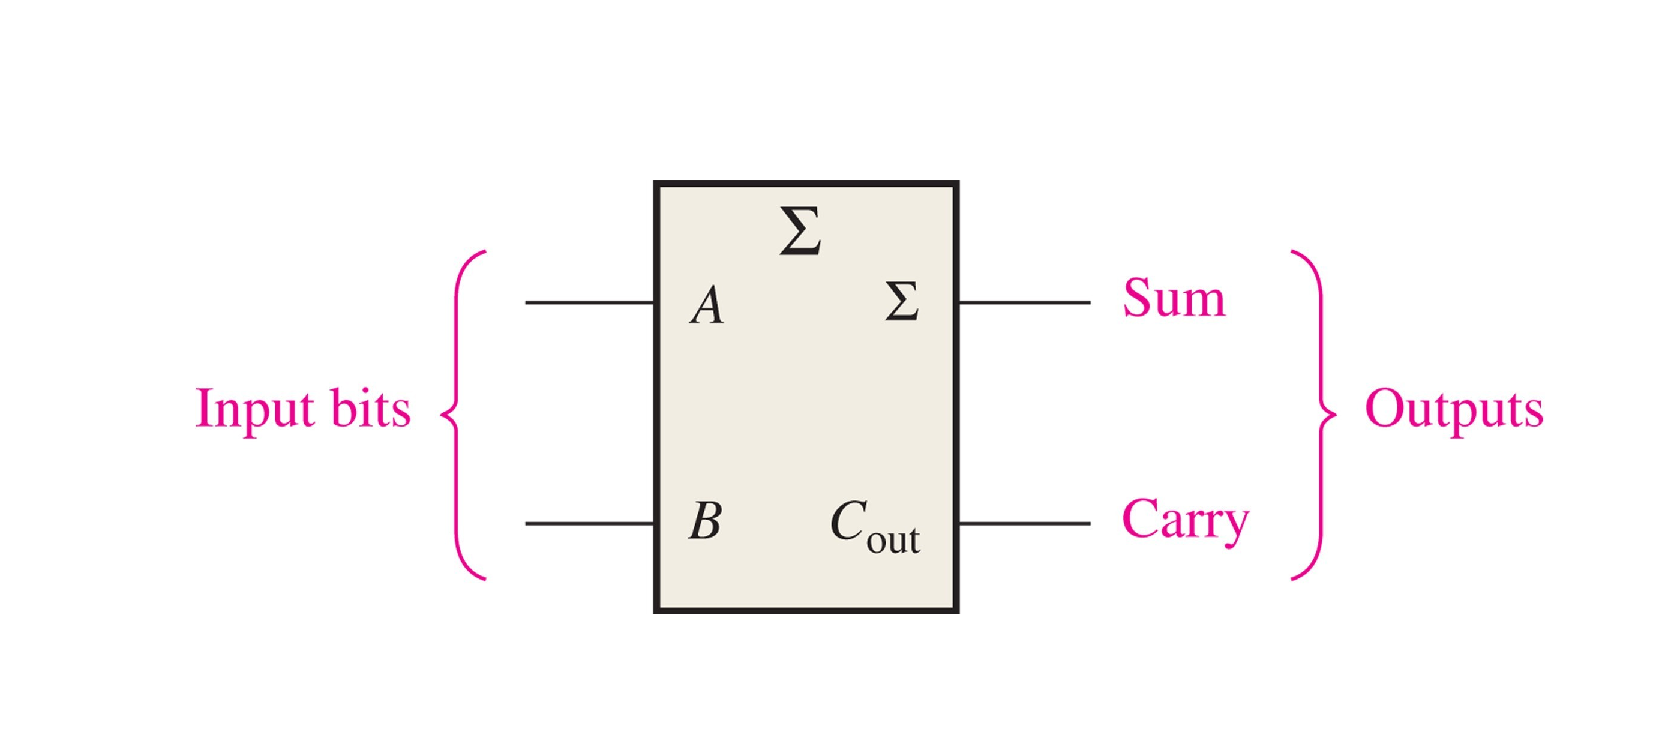
\includegraphics[width=0.9\textwidth]{figures/adder1.pdf}
\caption{\label{fig:add1} The desired inputs and outputs of the half-adder.  There is no carry-input.}
\end{figure}
\end{frame}

\begin{frame}{Half-Adders and Full-Adders, Ripple-Carry}
\begin{figure}
\centering
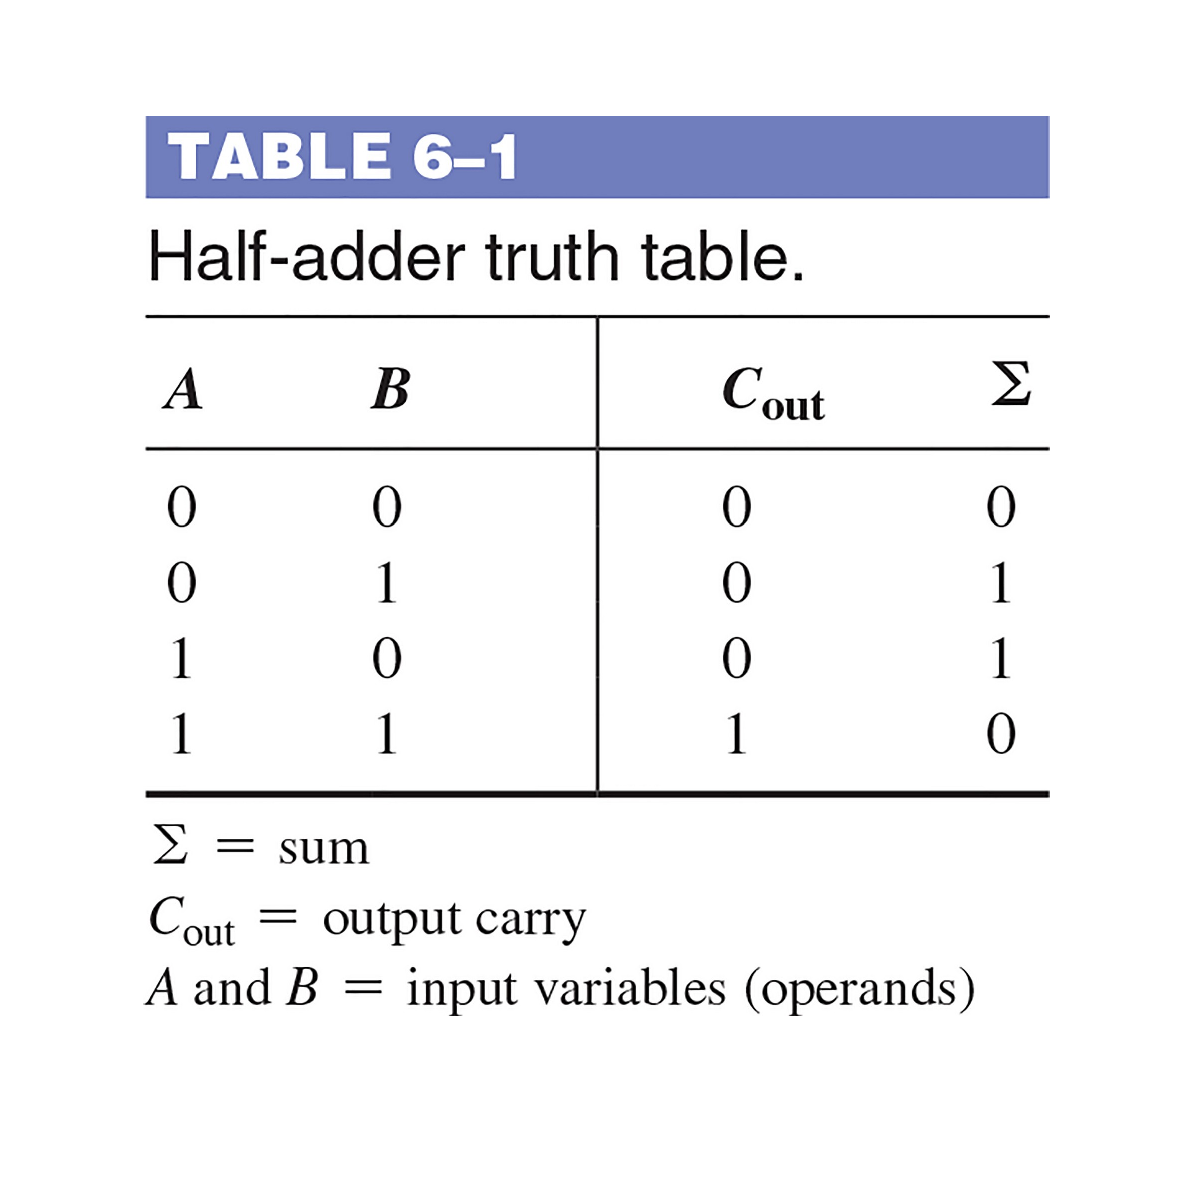
\includegraphics[width=0.5\textwidth]{figures/adder2.pdf}
\caption{\label{fig:add2} The truth table of the half-adder for 2-bits.  What gate action does this match?}
\end{figure}
\end{frame}

\begin{frame}{Half-Adders and Full-Adders, Ripple-Carry}
\begin{figure}
\centering
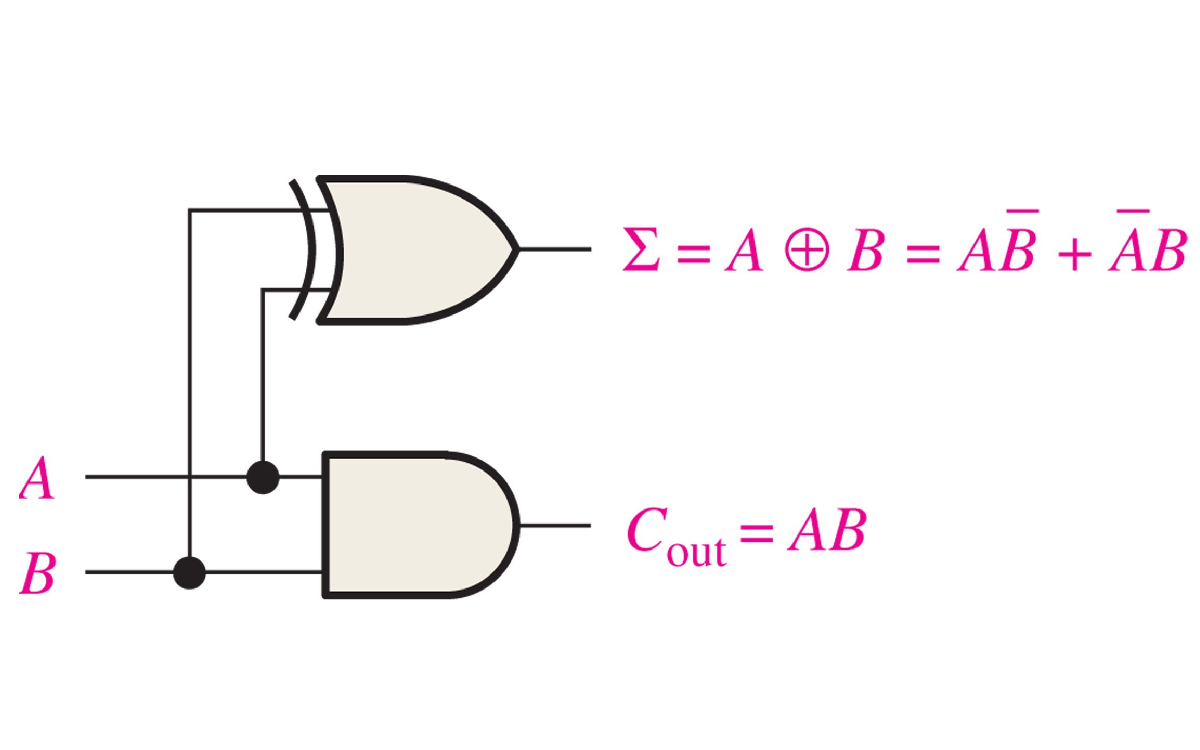
\includegraphics[width=0.7\textwidth]{figures/adder3.pdf}
\caption{\label{fig:add3} The logic function circuit diagram for the half-adder.}
\end{figure}
\end{frame}

\begin{frame}{Half-Adders and Full-Adders, Ripple-Carry}
\begin{figure}
\centering
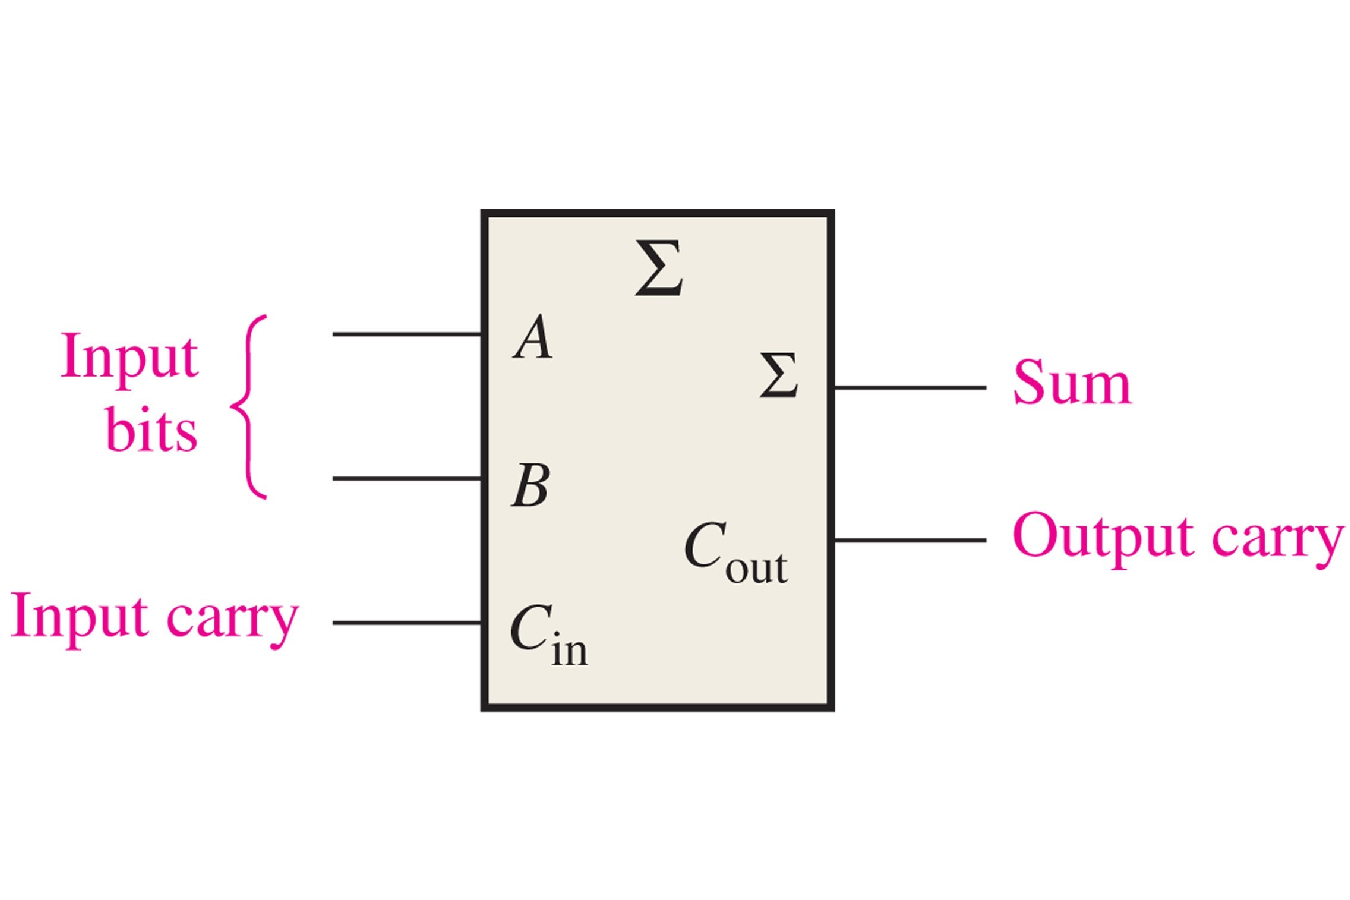
\includegraphics[width=0.7\textwidth]{figures/adder4.pdf}
\caption{\label{fig:add4} The desired inputs and outputs for the full-adder, with carry-input and carry-output.}
\end{figure}
\end{frame}

\begin{frame}{Half-Adders and Full-Adders, Ripple-Carry}
\begin{figure}
\centering
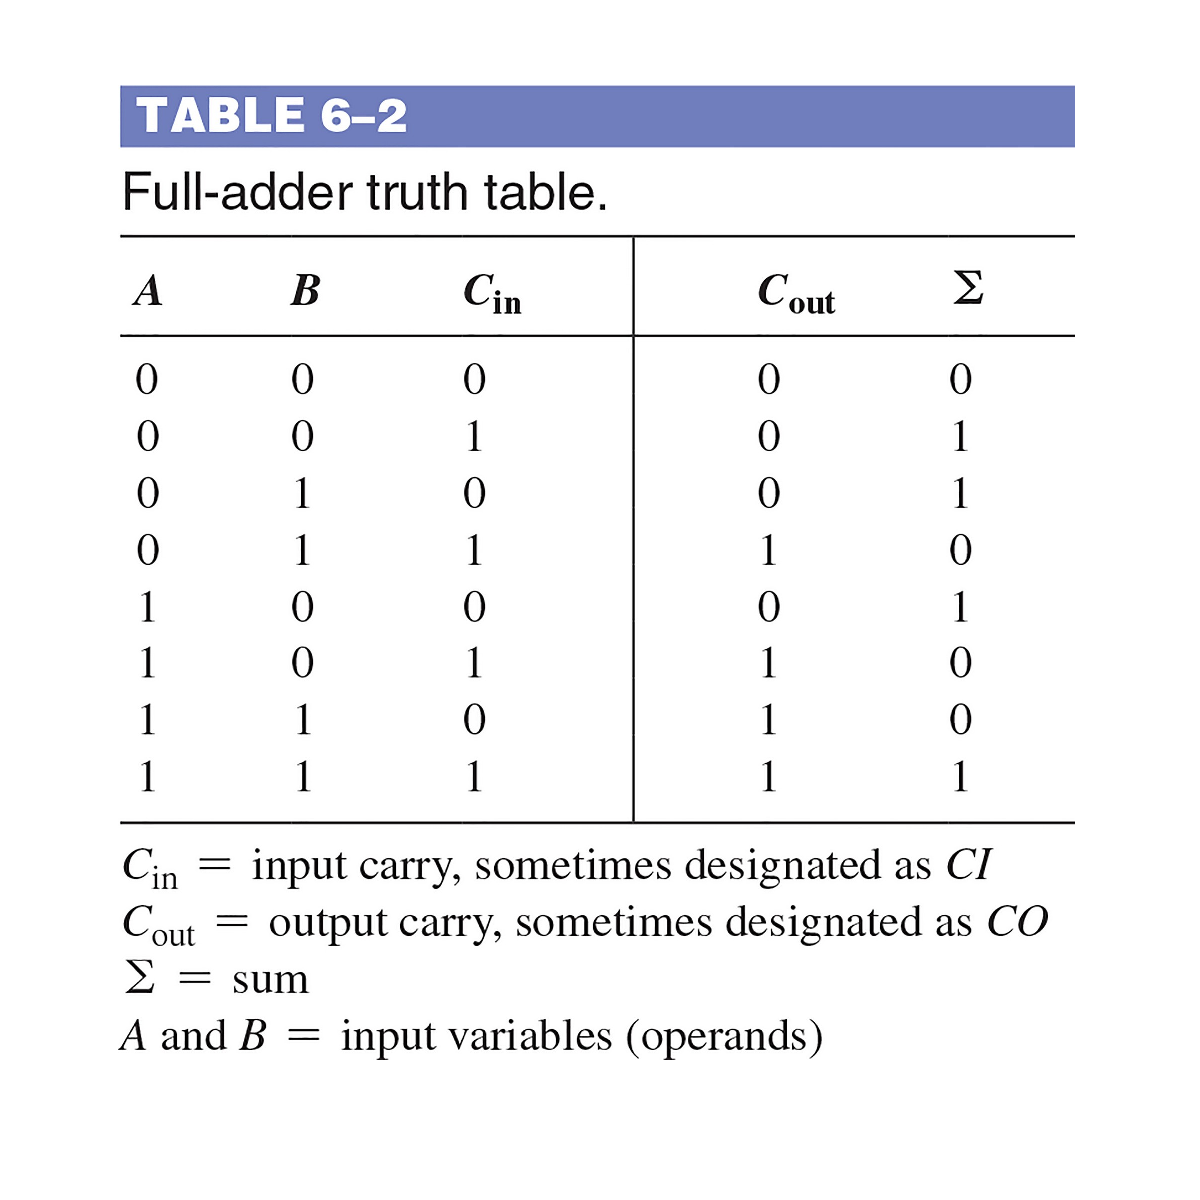
\includegraphics[width=0.5\textwidth]{figures/adder5.pdf}
\caption{\label{fig:add5} The truth table for the full-adder is more complex due to the increased number of inputs.}
\end{figure}
\end{frame}

\begin{frame}{Half-Adders and Full-Adders, Ripple-Carry}
\begin{figure}
\centering
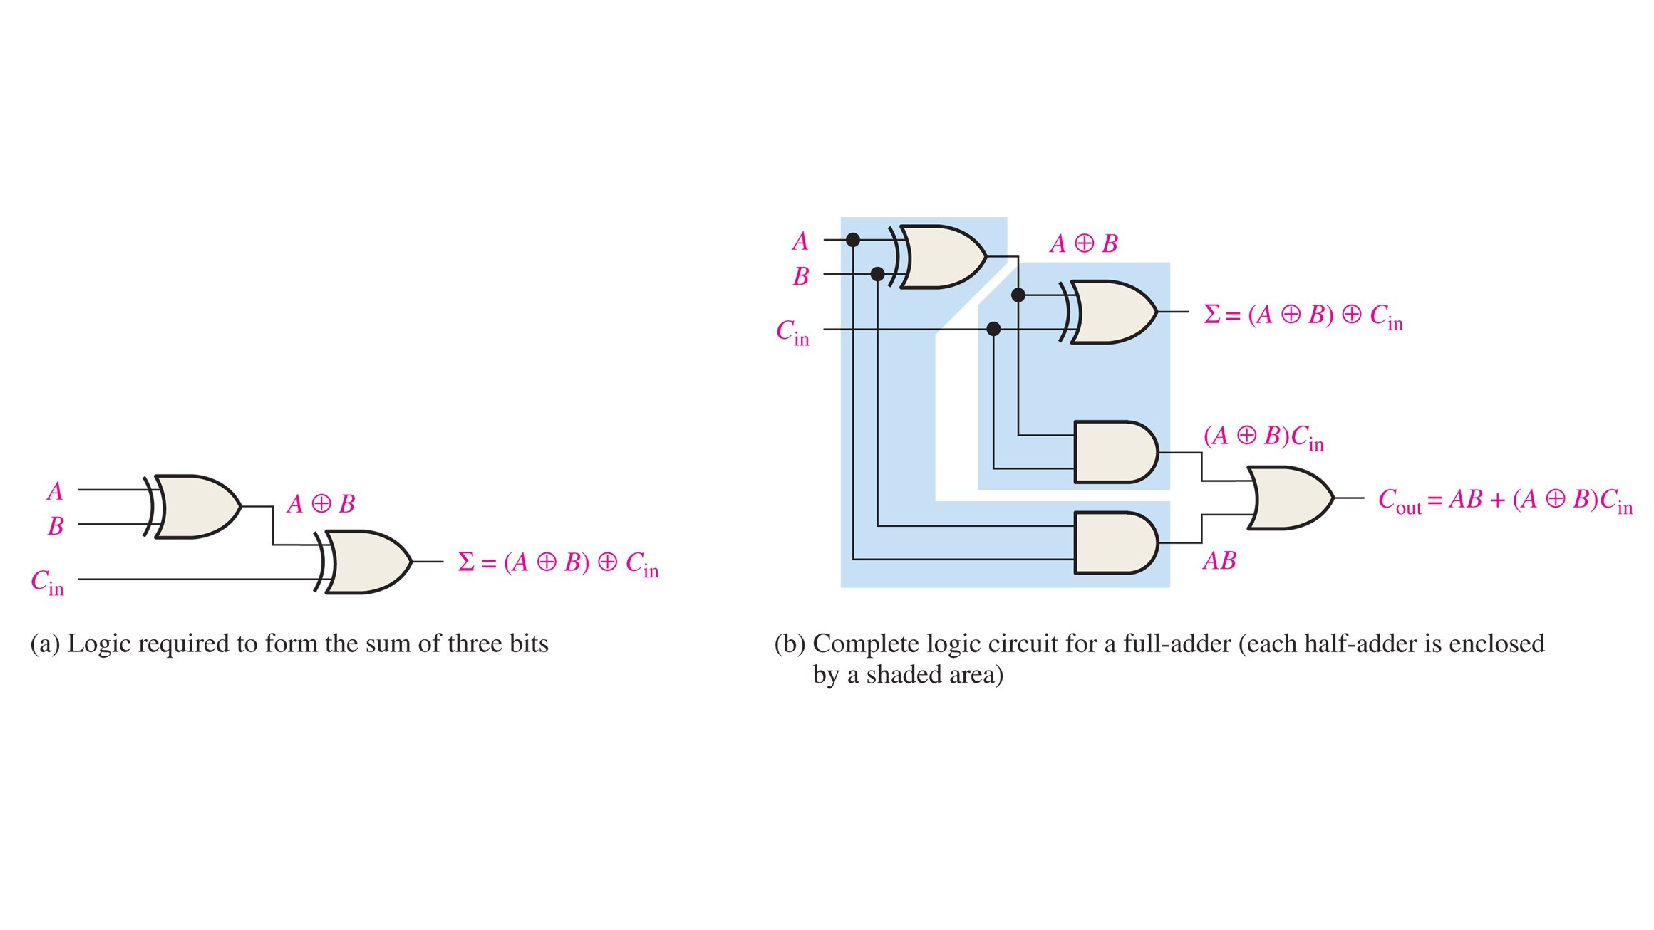
\includegraphics[width=0.9\textwidth]{figures/adder6.pdf}
\caption{\label{fig:add6} Circuit diagrams for the half-adder (left) and full-adder (right).}
\end{figure}
\end{frame}

\begin{frame}{Half-Adders and Full-Adders, Ripple-Carry}
\begin{figure}
\centering
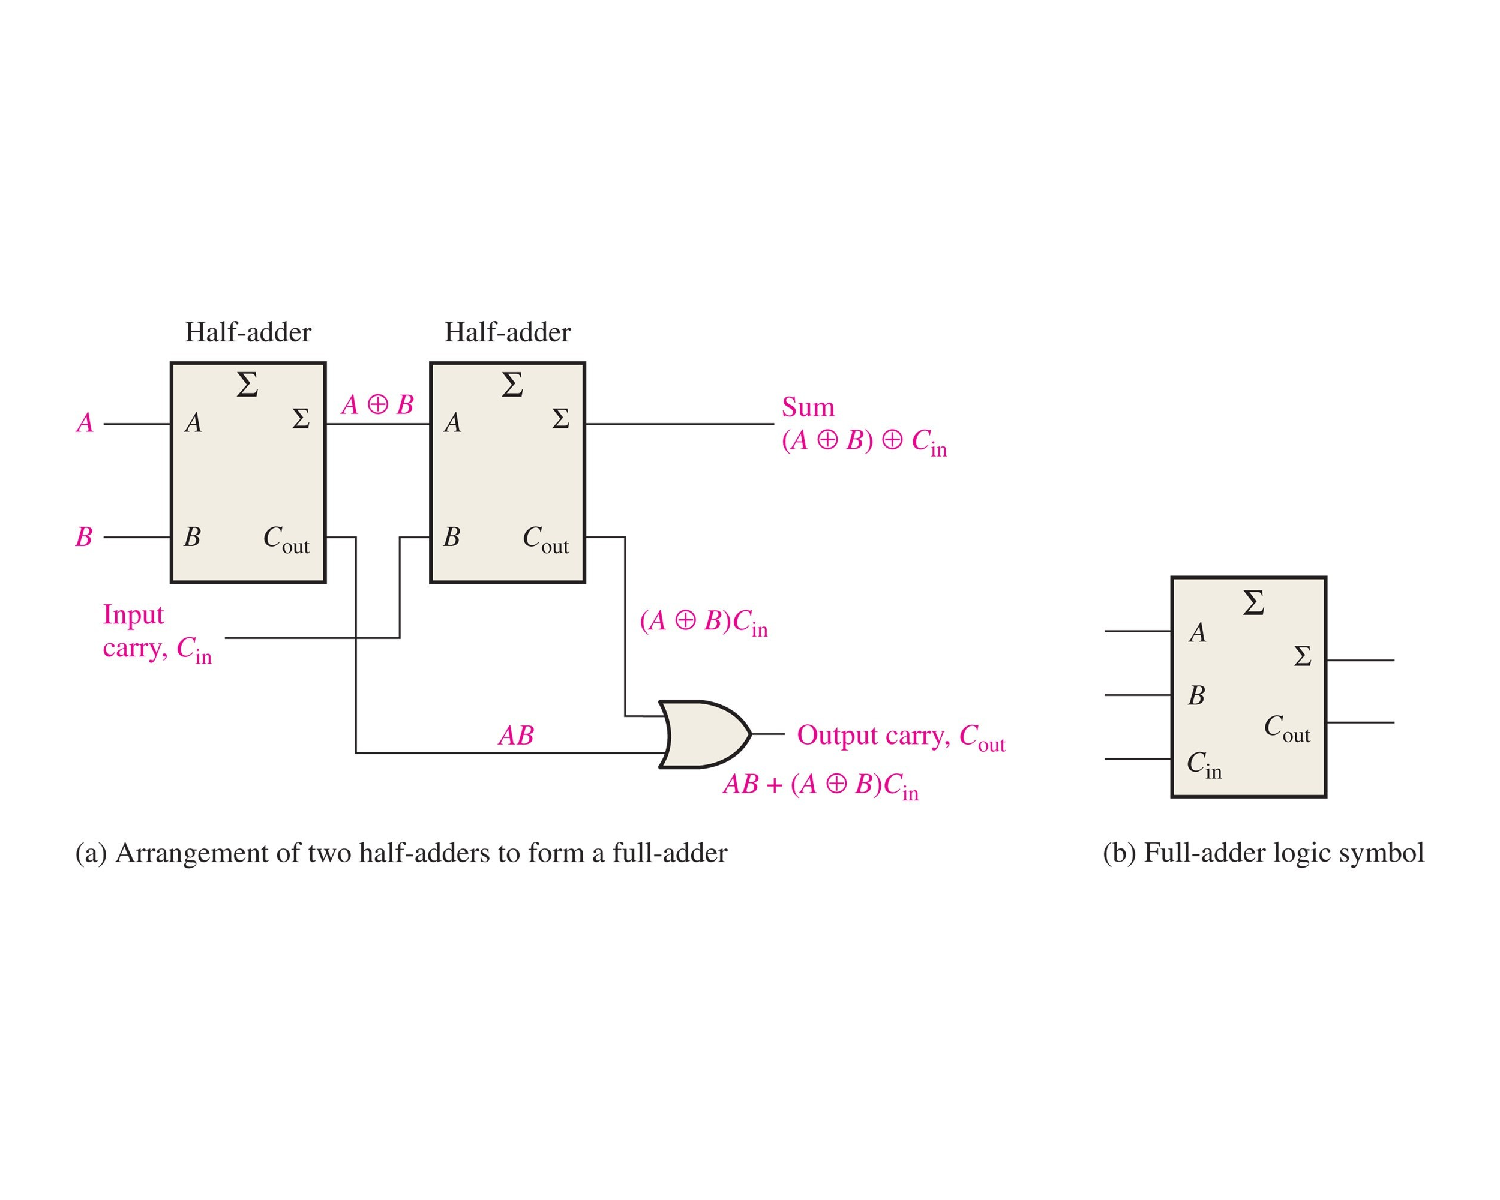
\includegraphics[width=0.7\textwidth]{figures/adder7.pdf}
\caption{\label{fig:add7} Two half-adders to form a full-adder.}
\end{figure}
\end{frame}

\begin{frame}{Half-Adders and Full-Adders, Ripple-Carry}
\begin{figure}
\centering
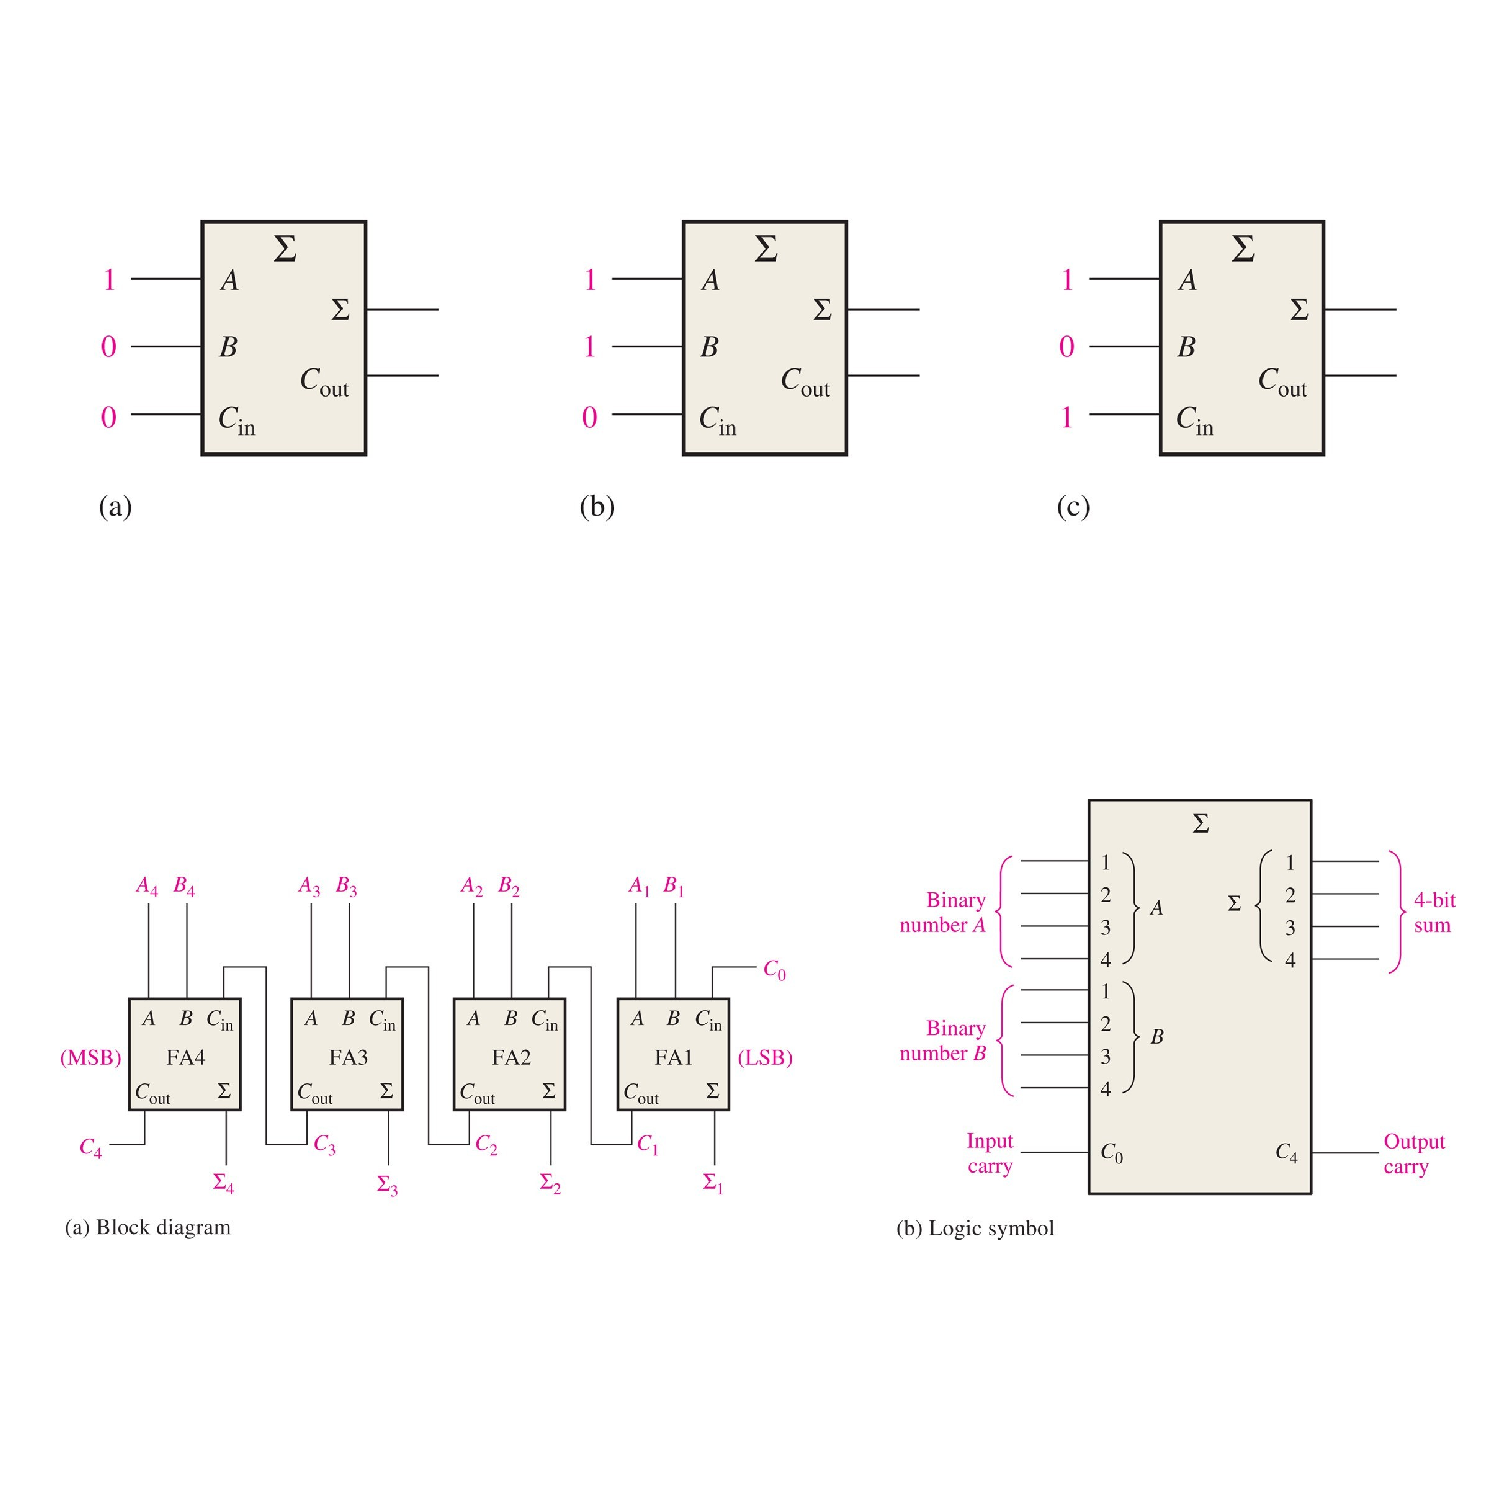
\includegraphics[width=0.5\textwidth]{figures/adder8.pdf}
\caption{\label{fig:add8} Four FA (full-adders) to add bits to the numbers being added.}
\end{figure}
\end{frame}

\begin{frame}{Half-Adders and Full-Adders, Ripple-Carry}
\begin{figure}
\centering
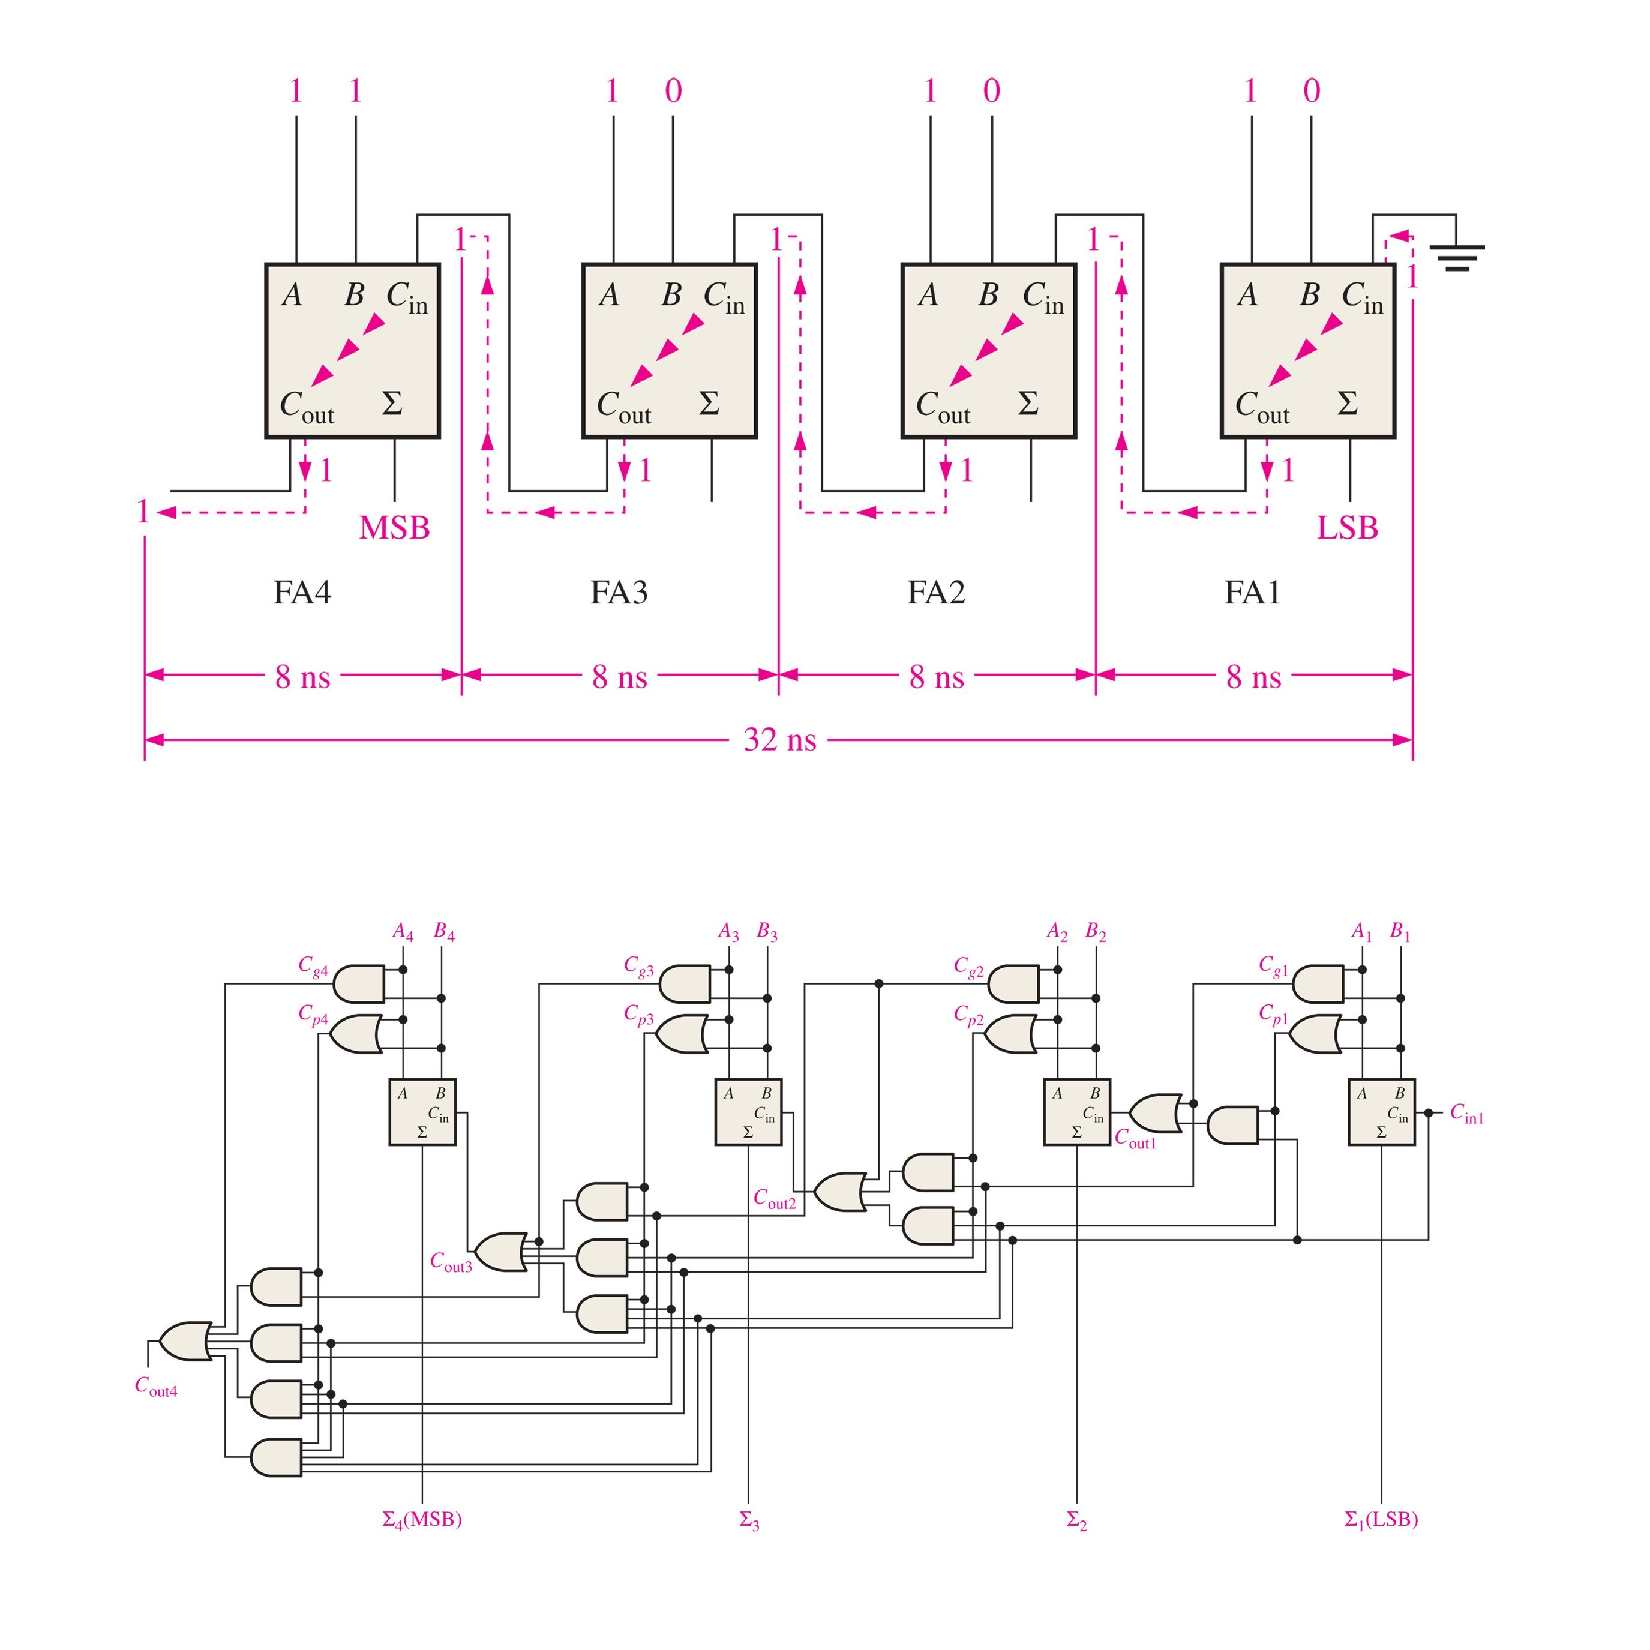
\includegraphics[width=0.5\textwidth]{figures/adder9.pdf}
\caption{\label{fig:add9} Propagation delays add serially in a full-adder with ripple carry topology.}
\end{figure}
\end{frame}

\section{Conclusion}

\begin{frame}{Unit 3 Summary}
\alert{Functions of Combinatorial Logic} \\
\textbf{Reading:} 6-1 - 6-6 (Tuesday) \\
\textbf{Reading:} 6-7 - 6-11 (Thursday)
\begin{enumerate}
\item Half-Adders and Full-Adders
\begin{itemize}
\item Example from study guide
\item Propagation delays
\end{itemize}
\item Comparators
\item Decodors/Encoders
\end{enumerate}
\end{frame}

\end{document}
